\chapter{Base Experiment}
\label{ch:Base_Experiment}

This chapter describes the base experiment, which serves the purpose of applying the approach and probing the hypothesis, presented in Chapter \ref{ch:Methodology}. A summarized representation of the workflow can be seen in Fig. \ref{fig:base_workflow}. In the following, we outline the steps for executing the experiment and the results of the evaluation.

\begin{figure}[!htb]
  \centering
  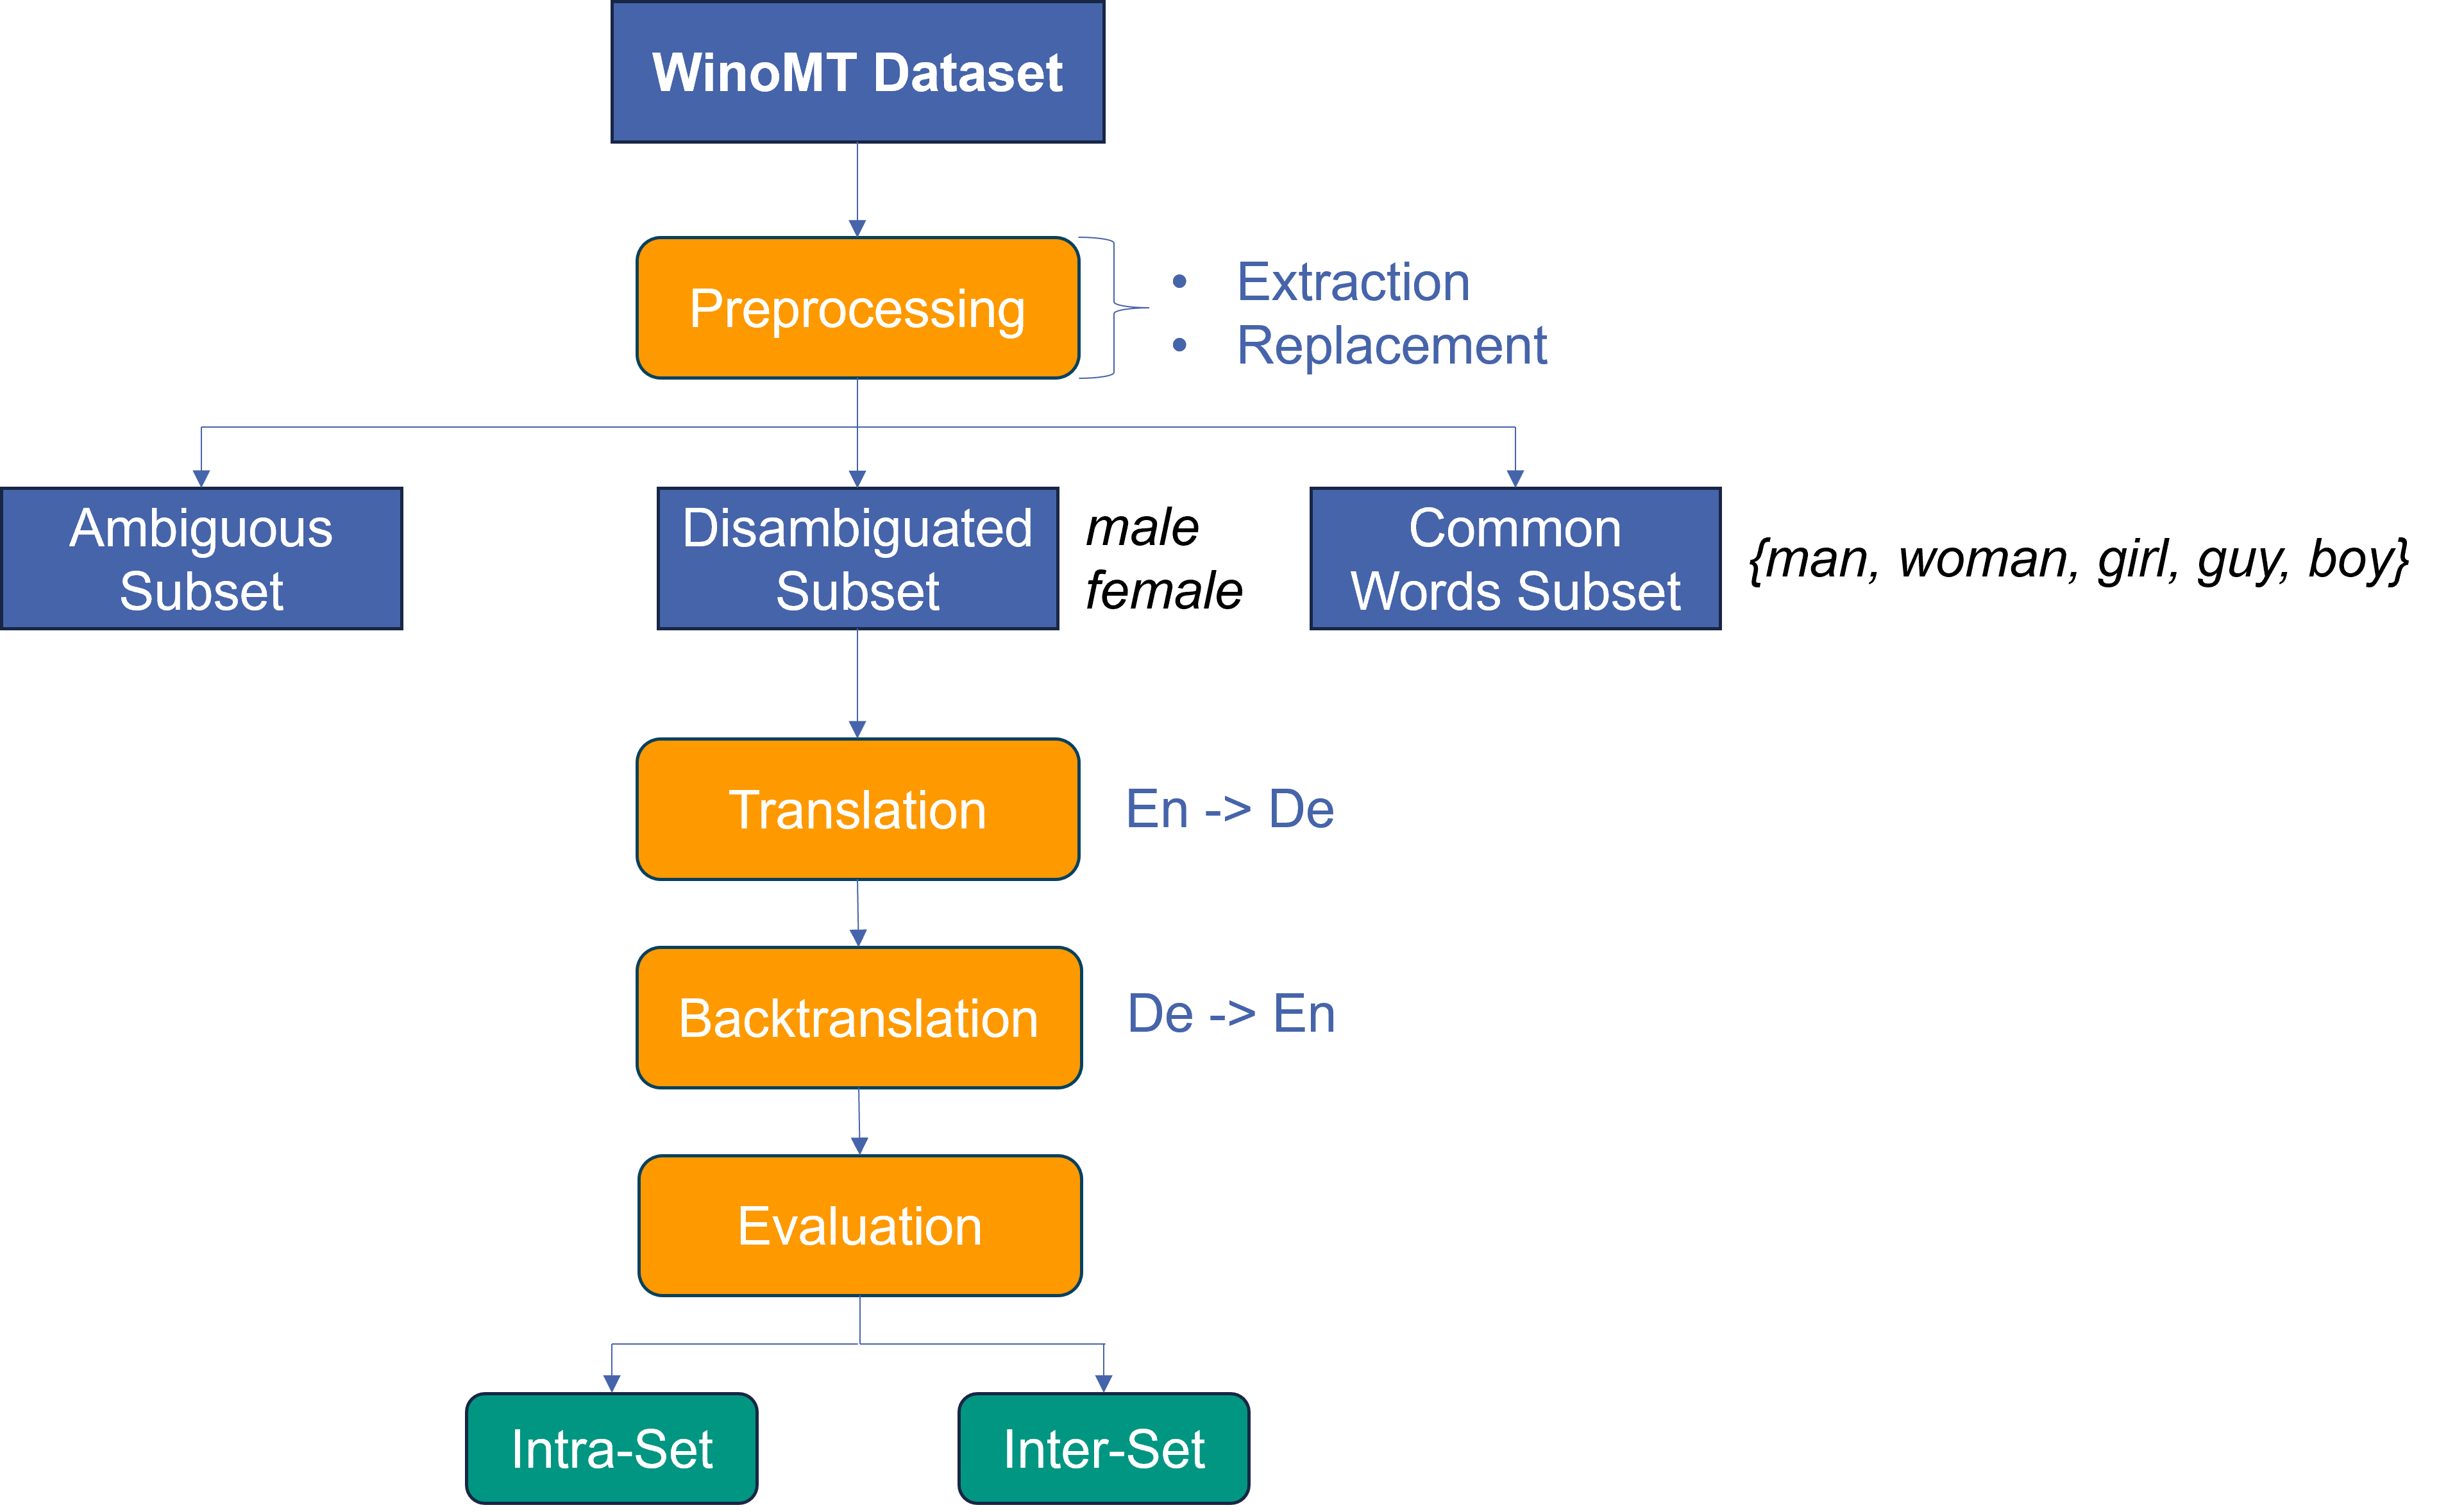
\includegraphics[scale=0.55]{figures/base_workflow.png}
  \caption{Base Experiment Workflow}
  \label{fig:base_workflow}
\end{figure}

%%%%%%%%%%%%%%%%%%%%%%%%%%%%%%%%%%%%%%%%%%%%%%%%%%%%%%%%%%%%%%%%%%%%%%%%%%%%%%%%%%%%%%%%%%%%
\section{Data Pre-processing}
\label{sec:Base_Experiment:Pre-processing}
The first step in conducting the base experiment is preprocessing the dataset. We use the artificially created WinoMT challenge set, presented in Subsection \ref{sec:Setup:Challenge_Set}. The sentences in this dataset usually consist of two gender-ambiguous occupation nouns and a context, containing disambiguation information about one of the occupations. We take the following steps to preprocess the sentences:

\begin{enumerate}
  \item \textbf{Sentence Extraction:}  
  In order to obtain fully ambiguous sentences, we remove the context information from the sentences and obtain a subset of 335 sentences from the type: "The developer argued with the designer.".
  To remove additional detection overhead, we want to have a single ambiguous word per sentence. For this purpose, we replace the second ambiguous word with a non-ambiguous proper noun, e.g., "John". 
  \item \textbf{Replacement:} As next, we generate new subsets of sentences, substituting the ambiguous word in the original sentence with a non-ambiguous version, using two different techniques:
  \begin{itemize}
      \item \textbf{Disambiguation:} We use the gender-defining adjectives \textit{male} and \textit{female} in front of the gender-ambiguous word. This technique is meant to force the translator to make the right decision regarding gender. % gender forcing
      \item \textbf{Common Words:} We replace the ambiguous word with each of the following common gender non-ambiguous words: \textit{man, woman, girl, guy, boy}. We evaluate for each word separately, as well as take the average of them. This method serves as a baseline for comparison against the disambiguated occupation nouns.
  \end{itemize}
\end{enumerate}

Table \ref{tab:preprocessing} shows the generated non-ambiguous subsets obtained by modifying the base ambiguous sentence "The developer argued with John.".

\begin{table}[!htb]
    \begin{tabularx}{\linewidth}{|l|X|l|}
        \hline
        \textbf{Replacement Method} & \textbf{Source Sentence} & \textbf{Source Word} \\ \hline
        \multirow{2}{*}{Disambiguation} & The \textbf{male developer} argued with John. & developer \\
        & The \textbf{female developer} argued with John. & developer \\ \hline
        \multirow{5}{*}{Common Words} & The \textbf{man} argued with John. & man \\
        & The \textbf{woman} argued with John. & woman \\
        & The \textbf{girl} argued with John. & girl \\
        & The \textbf{guy} argued with John. & guy \\
        & The \textbf{boy} argued with John. & boy \\ \hline
    \end{tabularx}
    \caption[Non-ambiguous subsets for the baseline sentence "The developer argued with John.".]{Non-ambiguous subsets for the baseline sentence "The developer argued with John.". \\ Source sentence: reflects the sentence in the non-ambiguous subset \\ Source word: word in the sentence we evaluate for}
    \label{tab:preprocessing}
\end{table}

The subsets resulting from the preprocessing are: 
\begin{itemize}
    \item \textbf{Ambiguous Subset}: a subset, containing the base ambiguous sentences.
    \item \textbf{Disambiguated Subset (male)}: a subset, containing the sentences, disambiguating the ambiguous word with \textit{male}.
    \item \textbf{Disambiguated Subset (female)}: a subset, containing the sentences, disambiguating the ambiguous word with \textit{female}.
    \item \textbf{Non-ambiguous Subsets}: five subsets, where the ambiguous word is replaced with the common words: \textit{man, woman, girl, guy, boy}.
\end{itemize}



%%%%%%%%%%%%%%%%%%%%%%%%%%%%%%%%%%%%%%%%%%%%%%%%%%%%%%%%%%%%%%%%%%%%%%%%%%%%%%%%%%%%%%%%%%%%
\section{Translation}
\label{sec:Base_Experiment:Translation}

The next step in conducting the experiments is translating the subsets of sentences. We translate from English to German. This is executed in two steps:

\begin{enumerate}
    \item \textbf{Translation Source -> Target:} 
    First, the subsets are translated in the target language (German).
    \item \textbf{Backtranslation Target -> Source:}
    The second step involves translating the translations back into the source language (English).
\end{enumerate}

For the purpose of  translation, we use two different decoding algorithms: Beam search and Sampling (see Subsection \ref{sec:Background:Decoding}). With Beam search, we compare the results for two different beam sizes: 10 and 100. The nbest size is the size of the number of unique translations, generated at each step. 

%%%%%%%%%%%%%%%%%%%%%%%%%%%%%%%%%%%%%%%%%%%%%%%%%%%%%%%%%%%%%%%%%%%%%%%%%%%%%%%%%%%%%%%%%%%%
\section{Word alignment}
\label{sec:Base_Experiment:Alignment}

\begin{figure}[!htb]
  \centering
  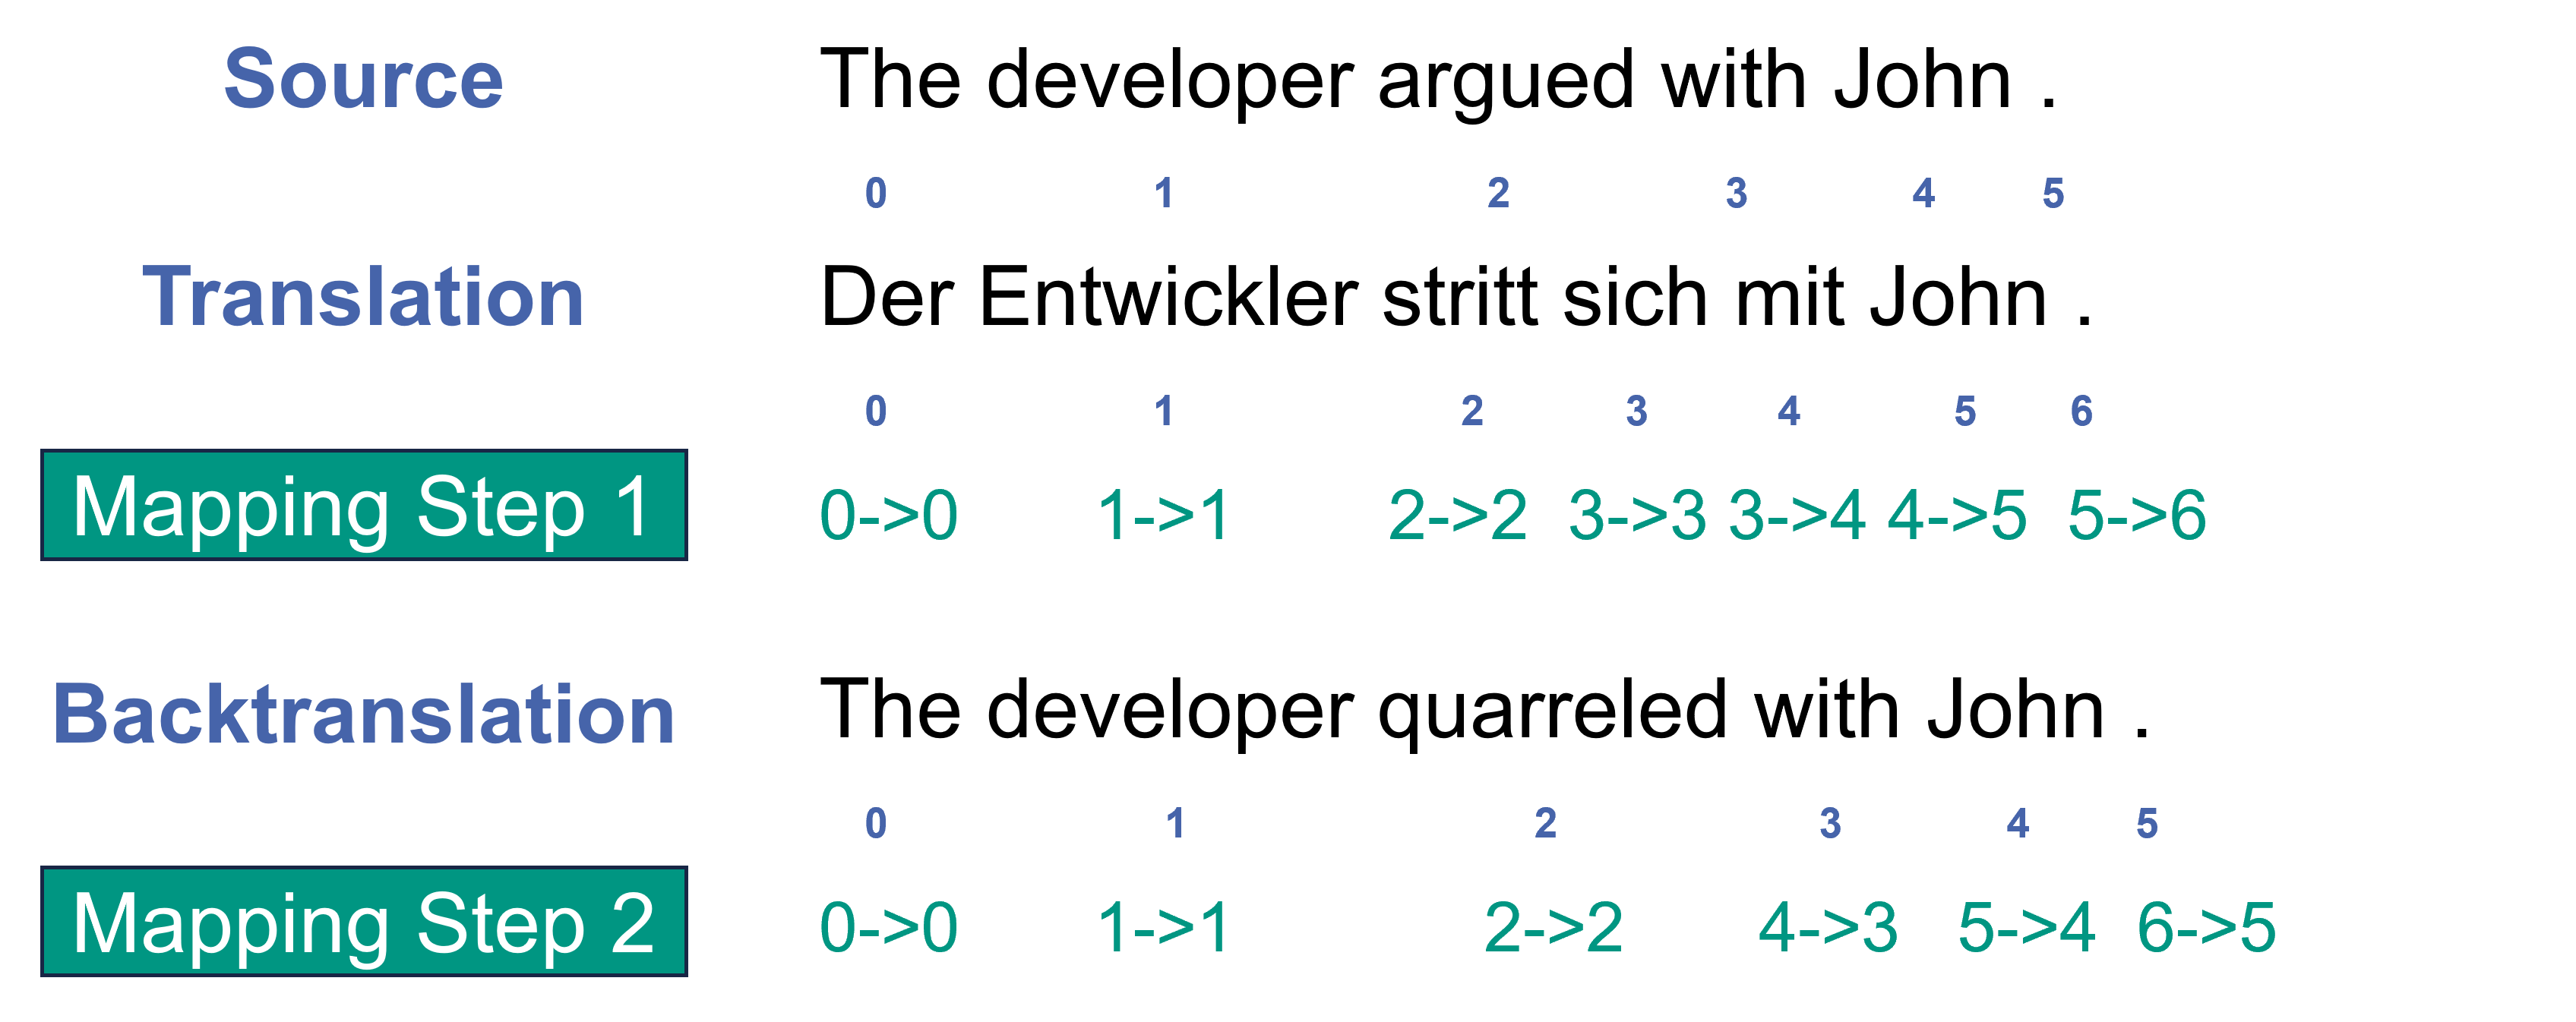
\includegraphics[scale=0.5]{figures/alignment.png}
  \caption{Example Illustration: 2-step mapping from source to translation and backtranslation}
  \label{fig:alignment}
\end{figure}

In order to assign the words in the source sentence to their counterparts in the translations, we use two different alignment methods:

\begin{itemize}
    \item Source-to-translation (\textit{fast\_align}, \textit{awesome-align}): This alignment method aligns from the source language to the target language.
    \item Translation-to-translation (\textit{Tercom}): This alignment method aligns between two translations.
\end{itemize}

We use the first method to map each word in the source sentence to its translations and backtranslations in the target nbest lists. We do this in a two-step way, depicted in Fig. \ref{fig:alignment}. First, we align between the source sentence and the sentences in the nbest translations and extract the translations for each word. Then, we align between the translations and the backtranslations and extract the corresponding backtranslations resulting from the aligned translations of each word. 

We use the results from the second method as a baseline for comparison with the first method and to detect possible errors, which may occur in the information transfer between the two steps in the first method.



%%%%%%%%%%%%%%%%%%%%%%%%%%%%%%%%%%%%%%%%%%%%%%%%%%%%%%%%%%%%%%%%%%%%%%%%%%%%%%%%%%%%%%%%%%%%
\section{Evaluation}
\label{sec:Base_Experiment:Evaluation}

The last step in the experiments involves evaluating the translations and backtranslations to detect patterns using different statistical methods. These methods aim to probe the initial Hypothesis \nameref{main}, discussed in Section \ref{sec:Methodology:Approach}. We apply all methods to all subsets, as presented in Section \ref{sec:Base_Experiment:Pre-processing}, and extract diversity information regarding the subsets themselves, as well as compare the results of the subsets against each other.

% define formally, maybe as a formula, pseudocode ???

%%%%%%%%%%%%%%%%%%%%%%%%%%%%%%%%%%%%%%%%%%%%%%%%%
\subsection{Reoccurrence Evaluation}
\label{sec:Base_Experiment:Statistics:Reoccurrence}
We evaluate how many of the source sentences and source words reoccur in the backtranslations:

\begin{enumerate}
    \item[1. ] Gather the backtranslations for each source sentences.
    \item[2a. ] Count the number of source sentences that reappear in their list of backtranslations.
    \item[2b. ] Count the number of source sentences which contain the source word in their backtranslations.
\end{enumerate}

% Is it to test which disambiguation method is better or to verify whether sentences in the ambiguous subset would be restore more often?
The purpose of this evaluation is to determine which of the subsets are able to reconstruct more of the source sentences/words. 

We also evaluate how often the source sentences and source words reoccur in the backtranslations:

\begin{enumerate}
    \item[1. ] Gather the backtranslations for each source sentences.
    \item[2a. ] Count in how many of the backtranslations the source sentences reappear.
    \item[2b. ] Count in how many of the backtranslations the source word reappears.
\end{enumerate}

We use both evaluations to verify whether sentences in the ambiguous subset would be restored more often than the disambiguated and the non-ambiguous subsets, with which we probe the Hypothesis \nameref{d}).

%%%%%%%%%%%%%%%%%%%%%%%%%%%%%%%%%%%%%%%%%%%%%%%%%
\subsection{Uniqueness Evaluation}
\label{sec:Base_Experiment:Statistics:Uniqueness}
We evaluate the number of unique words and sentences in the translations and backtranslations for each sentence of the subsets. 

For the sake of the evaluation, we follow this routine (\textit{[translations | backtranslations]} denotes that we follow the same step for both the translations and backtranslations):
\begin{enumerate}
    \item[1. ] Collect the \textit{[translations | backtranslations]} for each source sentences.
    % sentence level
    \item[2a. ] Count how many of the \textit{[translations | backtranslations]} are unique. 
    % word level
    \item[2b. ] Count how many unique words there are in the \textit{[translations | backtranslations]} and normalize the number by the total amount of words. 
    \item[3. ] Average the result for all sentences.
\end{enumerate}

We use this method to probe the Hypotheses \nameref{a}) and \nameref{b}). 

%%%%%%%%%%%%%%%%%%%%%%%%%%%%%%%%%%%%%%%%%%%%%%%%%
\subsection{Gender Evaluation}
\label{sec:Base_Experiment:Statistics:Gender}
We perform the evaluation of gender on the translations of the subsets.  First, we align each word in the source sentence with its corresponding word in the translations and backtranslations (see Subsection \ref{sec:Base_Experiment:Alignment} for more detail). Then, we perform the following steps:

\begin{enumerate}
    \item[1. ] Gather the translations of the source word for each source sentence.
    \item[2. ] Detect the gender of the translations for each source sentence.
    \item[3a. ] Determine the proportion of source sentences producing \textit{male} versus \textit{female}.
    \item[3b. ] Calculate how many of the source sentences produce \textit{both genders}. 
\end{enumerate}

The purpose of this method is to assess if the translations produce the right gender (in the non-ambiguous subsets) or both genders (in the ambiguous subset) and how often they produce both genders for each subset.

%%%%%%%%%%%%%%%%%%%%%%%%%%%%%%%%%%%%%%%%%%%%%%%%%
\subsection{Alignment Evaluation}
\label{sec:Base_Experiment:Statistics:Alignment}
Another form of evaluation is based on the alignment of the words between the source sentence, the translations and backtranslations (see Subsection \ref{sec:Base_Experiment:Alignment} for more detail).

In order to assess the translations and backtranslations of the \textbf{source word}, we do:
\begin{enumerate}
    \item[1. ] Collect all \textit{[translations | backtranslations]} of the source word.
    \item[2. ] Count how many of the \textit{[translations | backtranslations]} are unique.
    \item[3. ] Average the result for all sentences.
\end{enumerate}

Similarly, to assess the translations and backtranslations of the \textbf{rest of the sentence} excluding the source word, we do:
\begin{enumerate}
    \item[1. ] Collect all \textit{[translations | backtranslations]} of the sentence rest.
    \item[2. ] Count how many of the \textit{[translations | backtranslations]} are unique.
    \item[3. ] Average the result for all sentences.
\end{enumerate}

The idea behind this evaluation method is to assess the Hypothesis \nameref{c}).

Next, we will present the results of these statistical evaluations of the subsets.

